\documentclass{article}
\usepackage[utf8]{inputenc}
\usepackage[spanish]{babel}
\usepackage{amsmath}
\usepackage{amsfonts}
\usepackage{amssymb}
\usepackage{graphicx}
\usepackage{float}
\usepackage{hyperref}
\bibliographystyle{plain}

%opening
\title{Actividad 1: Análisis Matemático de Funciones}
\author{Sergio Andrés Elizondo Rodríguez}
\date{20 de Septiembre del 2024}

\begin{document}

\maketitle

\section*{Problema 1: Análisis de la Función \( f(x) = x^3 - 6x \)}

\subsection*{a) Obtención de los Puntos Críticos}
Consideremos la función \( f: \mathbb{R} \to \mathbb{R} \) definida por:
\[
f(x) = x^3 - 6x.
\]

Para determinar los puntos críticos de la función, es necesario resolver la ecuación \( f'(x) = 0 \), donde \( f'(x) \) es la derivada de \( f(x) \).

Calculamos la derivada:
\[
f'(x) = \frac{d}{dx}(x^3 - 6x) = 3x^2 - 6.
\]

Igualamos la derivada a cero para encontrar los puntos críticos:
\[
f'(x) = 3x^2 - 6 = 0.
\]

Resolviendo la ecuación:
\[
3x^2 - 6 = 0 \iff x^2 = 2 \iff x = \pm\sqrt{2}.
\]

Por lo tanto, los puntos críticos son
\[
x_1 = \sqrt{2} \quad \text{y} \quad x_2 = -\sqrt{2}.
\]

\subsection*{b) Clasificación de los Puntos Críticos}
Para clasificar los puntos críticos obtenidos, se requiere calcular la segunda derivada de \( f(x) \):
\[
f''(x) = \frac{d}{dx}(3x^2 - 6) = 6x.
\]

A continuación, evaluamos la segunda derivada en los puntos críticos:
\begin{enumerate}
	\item Para \( x = \sqrt{2} \):
	\[
	f''(\sqrt{2}) = 6\sqrt{2} > 0.
	\]
	
	Por lo tanto, \( x_1 = \sqrt{2} \) es un mínimo local.
	
	\item Para \( x = -\sqrt{2} \):
	\[
	f''(-\sqrt{2}) = 6(-\sqrt{2}) < 0.
	\]
	
	Por lo tanto, \( x_2 = -\sqrt{2} \) es un máximo local.
\end{enumerate}

Para encontrar los puntos de inflexión, igualamos la segunda derivada a cero:
\[
f''(x) = 6x = 0 \implies x = 0.
\]

\subsection*{c) Gráfica de $f(x)$}

\begin{figure}[h]
	\centering
	\includegraphics[width=0.8\textwidth]{graficas/grafica_2d.png}
	\caption{Gráfica de la función \( f(x) = x^3 - 6x \) y sus puntos críticos.}
	\label{fig:grafica_funcion}
\end{figure}

Para graficar la función, determinamos los valores de \( f(x) \) en los puntos críticos y en el punto de inflexión:
\begin{enumerate}
	\item Para \( x = -\sqrt{2} \):
	\[
	f(-\sqrt{2}) = (-\sqrt{2})^3 - 6(-\sqrt{2}) = -2\sqrt{2} + 6\sqrt{2} = 4\sqrt{2}.
	\]
	
	\item Para \( x = \sqrt{2} \):
	\[
	f(\sqrt{2}) = (\sqrt{2})^3 - 6\sqrt{2} = 2\sqrt{2} - 6\sqrt{2} = -4\sqrt{2}.
	\]
	
	\item Para \( x = 0 \):
	\[
	f(0) = 0^3 - 6(0) = 0.
	\]
\end{enumerate}

En la figura \ref{fig:grafica_funcion} se muestra la gráfica de la función \( f(x) = x^3 - 6x \) y sus puntos críticos.\cite{Elizondo2024}

\subsection*{d) Análisis de Crecimiento, Decrecimiento y Concavidad}
\begin{enumerate}
	\item \textbf{Crecimiento y Decrecimiento}
	
	La función \( f(x) \) es creciente cuando \( f'(x) > 0 \):
	\[
	3x^2 - 6 > 0 \iff x^2 > 2 \iff x < -\sqrt{2} \quad \text{ó} \quad x > \sqrt{2}.
	\]
	
	La función \( f(x) \) es decreciente cuando \( f'(x) < 0 \):
	\[
	-\sqrt{2} < x < \sqrt{2}.
	\]
	
	\item \textbf{Concavidad}
	
	La función \( f(x) \) es cóncava hacia arriba cuando \( f''(x) > 0 \):
	\[
	6x > 0 \iff x > 0.
	\]
	
	La función \( f(x) \) es cóncava hacia abajo cuando \( f''(x) < 0 \):
	\[
	6 x < 0 \iff x < 0.
	\]
\end{enumerate}

\subsection*{Conclusión}
El análisis realizado sobre la función \( f(x) = x^3 - 6x \) revela la existencia de un máximo local en \( (-\sqrt{2}, 4\sqrt{2}) \), un mínimo local en \( (\sqrt{2}, -4\sqrt{2}) \) y un punto de inflexión en \( (0, 0) \). Además, se determinó que la función crece en los intervalos \( (-\infty, -\sqrt{2}) \) y \( (\sqrt{2}, \infty) \), mientras que decrece en el intervalo \( (-\sqrt{2}, \sqrt{2}) \). Finalmente, la función es cóncava hacia arriba para \( x > 0 \) y hacia abajo para \( x < 0 \).

\newpage

\section*{Problema 2: Análisis de la Función \(f(x, y) = x^2 + y^2 + 4xy\)}

\subsection*{a) Obtención de los Puntos Críticos}

Consideremos la función \( f : \mathbb{R}^2 \to \mathbb{R} \) definida por:
\[
f(x, y) = x^2 + y^2 + 4xy.
\]

Para determinar los puntos críticos de \( f(x, y) \), es necesario resolver el sistema de ecuaciones \( \nabla f = 0 \), donde \( \nabla f = (f_x, f_y) = \left( \frac{\partial f}{\partial x}, \frac{\partial f}{\partial y} \right) \) es el gradiente de la función y \( f_x \) y \( f_y \) son las derivadas parciales respecto a \( x \) e \( y \), respectivamente.

Calculamos la derivada parcial con respecto a \( x \):
\[
f_x = \frac{\partial}{\partial x}(x^2 + y^2 + 4xy) = 2x + 4y.
\]

Calculamos la derivada parcial con respecto a \( y \):
\[
f_y = \frac{\partial}{\partial y }(x^2 + y^2 + 4xy) = 2y + 4x.
\]

Igualamos ambas derivadas a cero para encontrar los puntos críticos:
\begin{enumerate}
	\item \( f_x = 2x + 4y = 0 \).
	\item \( f_y = 2y + 4x = 0 \).
\end{enumerate}

A partir de la primera ecuación, tenemos que
\[
2x + 4y = 0 \iff x = -2y.
\]

Sustituyendo \( x = -2y \) en la segunda ecuación:
\[
2y + 4(-2y) = 0 \iff 2y - 8y = 0 \iff -6y = 0 \iff y = 0.
\]

Sustituyendo \( y = 0 \) en \( x = -2y \):
\[
x = -2(0) = 0.
\]

Por lo tanto, el único punto crítico es
\[
(x_0, y_0) = (0, 0).
\]

\subsection*{b) Clasificación del Punto Crítico}
Para clasificar el punto crítico \( (0, 0) \), calculamos la matriz hessiana \( H \) de la función \( f(x, y) \):
\[
H = \begin{bmatrix}
	f_{xx} & f_{xy} \\
	f_{yx} & f_{yy}
\end{bmatrix}.
\]

Calculamos las segundas derivadas parciales:
\begin{enumerate}
	\item \( f_{xx} = \frac{\partial^2 f}{\partial x^2} = 2 \).
	\item \( f_{xy} = \frac{\partial^2 f}{\partial x \partial y} = 4 \).
	\item \( f_{yx} = \frac{\partial^2 f}{\partial y \partial x} = 4 \).
	\item \( f_{yy} = \frac{\partial^2 f}{\partial y^2} = 2 \).
\end{enumerate}

Por lo tanto, la matriz hessiana es
\[
H = \begin{bmatrix}
	2 & 4 \\
	4 & 2
\end{bmatrix}.
\]

Los valores propios del hessiano \( \lambda_1 \) y \( \lambda_2 \) indican la clasificación del punto crítico de la siguiente manera:
\begin{enumerate}
	\item Si ambos son positivos (\(\lambda_1 > 0 \) y \( \lambda_2 > 0 \)), el punto crítico es un \textbf{mínimo local}.
	\item Si ambos son negativos (\(\lambda_1 < 0 \) y \( \lambda_2 < 0 \)), el punto crítico es un \textbf{máximo local}.
	\item Si uno es positivo y otro negativo (\(\lambda_1 > 0 \) y \( \lambda_2 > 0 \) o viceversa), el punto crítico es un \textbf{punto silla}.
\end{enumerate}

Si el determinante de la matriz hessiana es negativo, es decir,
\[
\text{det}(H) < 0,
\]

esto implica que el producto de los valores propios es negativo:
\[
\lambda_1 \cdot \lambda_2 < 0.
\]

Esto sólo puede ocurrir si uno de los valores propios es positivo y el otro negativo:
\begin{itemize}
	\item \( \lambda_1 > 0 \) y \( \lambda_2 < 0 \) ó
	\item \( \lambda_1 < 0 \) y \( \lambda_2 > 0 \).
\end{itemize}

En ambos casos, esto cumple la condición para que el punto crítico sea un \textbf{punto silla}. Calculamos el determinante de \( H \):
\[
\text{det}(H) = (2)(2) - (4)(4) = 4 - 16 = -12.
\]

Dado que el determinante de la matriz hessiana es negativo, se concluye que el punto crítico \( (0, 0) \) es un punto silla.

\subsection*{c) Gráfica de $f(x)$}

En la figura \ref{fig:grafica_contorno} se muestra la gráfica de contorno de la función \( f(x) = x^3 - 6x \) y su punto crítico, mientras que en la figura \ref{fig:grafica_3d} se muestra su representación tridimensional.\cite{Elizondo2024}

\begin{figure}[h]
	\centering
	\includegraphics[width=0.8\textwidth]{graficas/grafica_contorno.png}
	\caption{Gráfica de contorno de \( f(x, y) = x^2 + y^2 + 4xy \) y su punto crítico.}
	\label{fig:grafica_contorno}
\end{figure}

\begin{figure}[H]
	\centering
	\includegraphics[width=0.8\textwidth]{graficas/grafica_3d.png}
	\caption{Gráfica tridimensional de \( f(x, y) = x^2 + y^2 + 4xy \) y su punto crítico.}
	\label{fig:grafica_3d}
\end{figure}

\subsection*{Conclusión}
El análisis realizado sobre la función \( f(x, y) = x^2 + y^2 + 4xy \) revela la existencia de un único punto crítico en \( (0, 0) \), clasificado como punto silla.

\section*{Procedimiento a mano}

% Imagen 1
\begin{figure}[H]
	\centering
	\includegraphics[width=0.8\textwidth]{imagenes/pagina1.png}
	\caption{Procedimiento a mano - Página 1}
	\label{fig:procedimiento_1}
\end{figure}

% Imagen 2
\begin{figure}[H]
	\centering
	\includegraphics[width=0.8\textwidth]{imagenes/pagina2.png}
	\caption{Procedimiento a mano - Página 2}
	\label{fig:procedimiento_2}
\end{figure}

% Imagen 3
\begin{figure}[H]
	\centering
	\includegraphics[width=0.8\textwidth]{imagenes/pagina3.png}
	\caption{Procedimiento a mano - Página 3}
	\label{fig:procedimiento_3}
\end{figure}

% Imagen 4
\begin{figure}[H]
	\centering
	\includegraphics[width=0.8\textwidth]{imagenes/pagina4.png}
	\caption{Procedimiento a mano - Página 4}
	\label{fig:procedimiento_4}
\end{figure}

% Imagen 5
\begin{figure}[H]
	\centering
	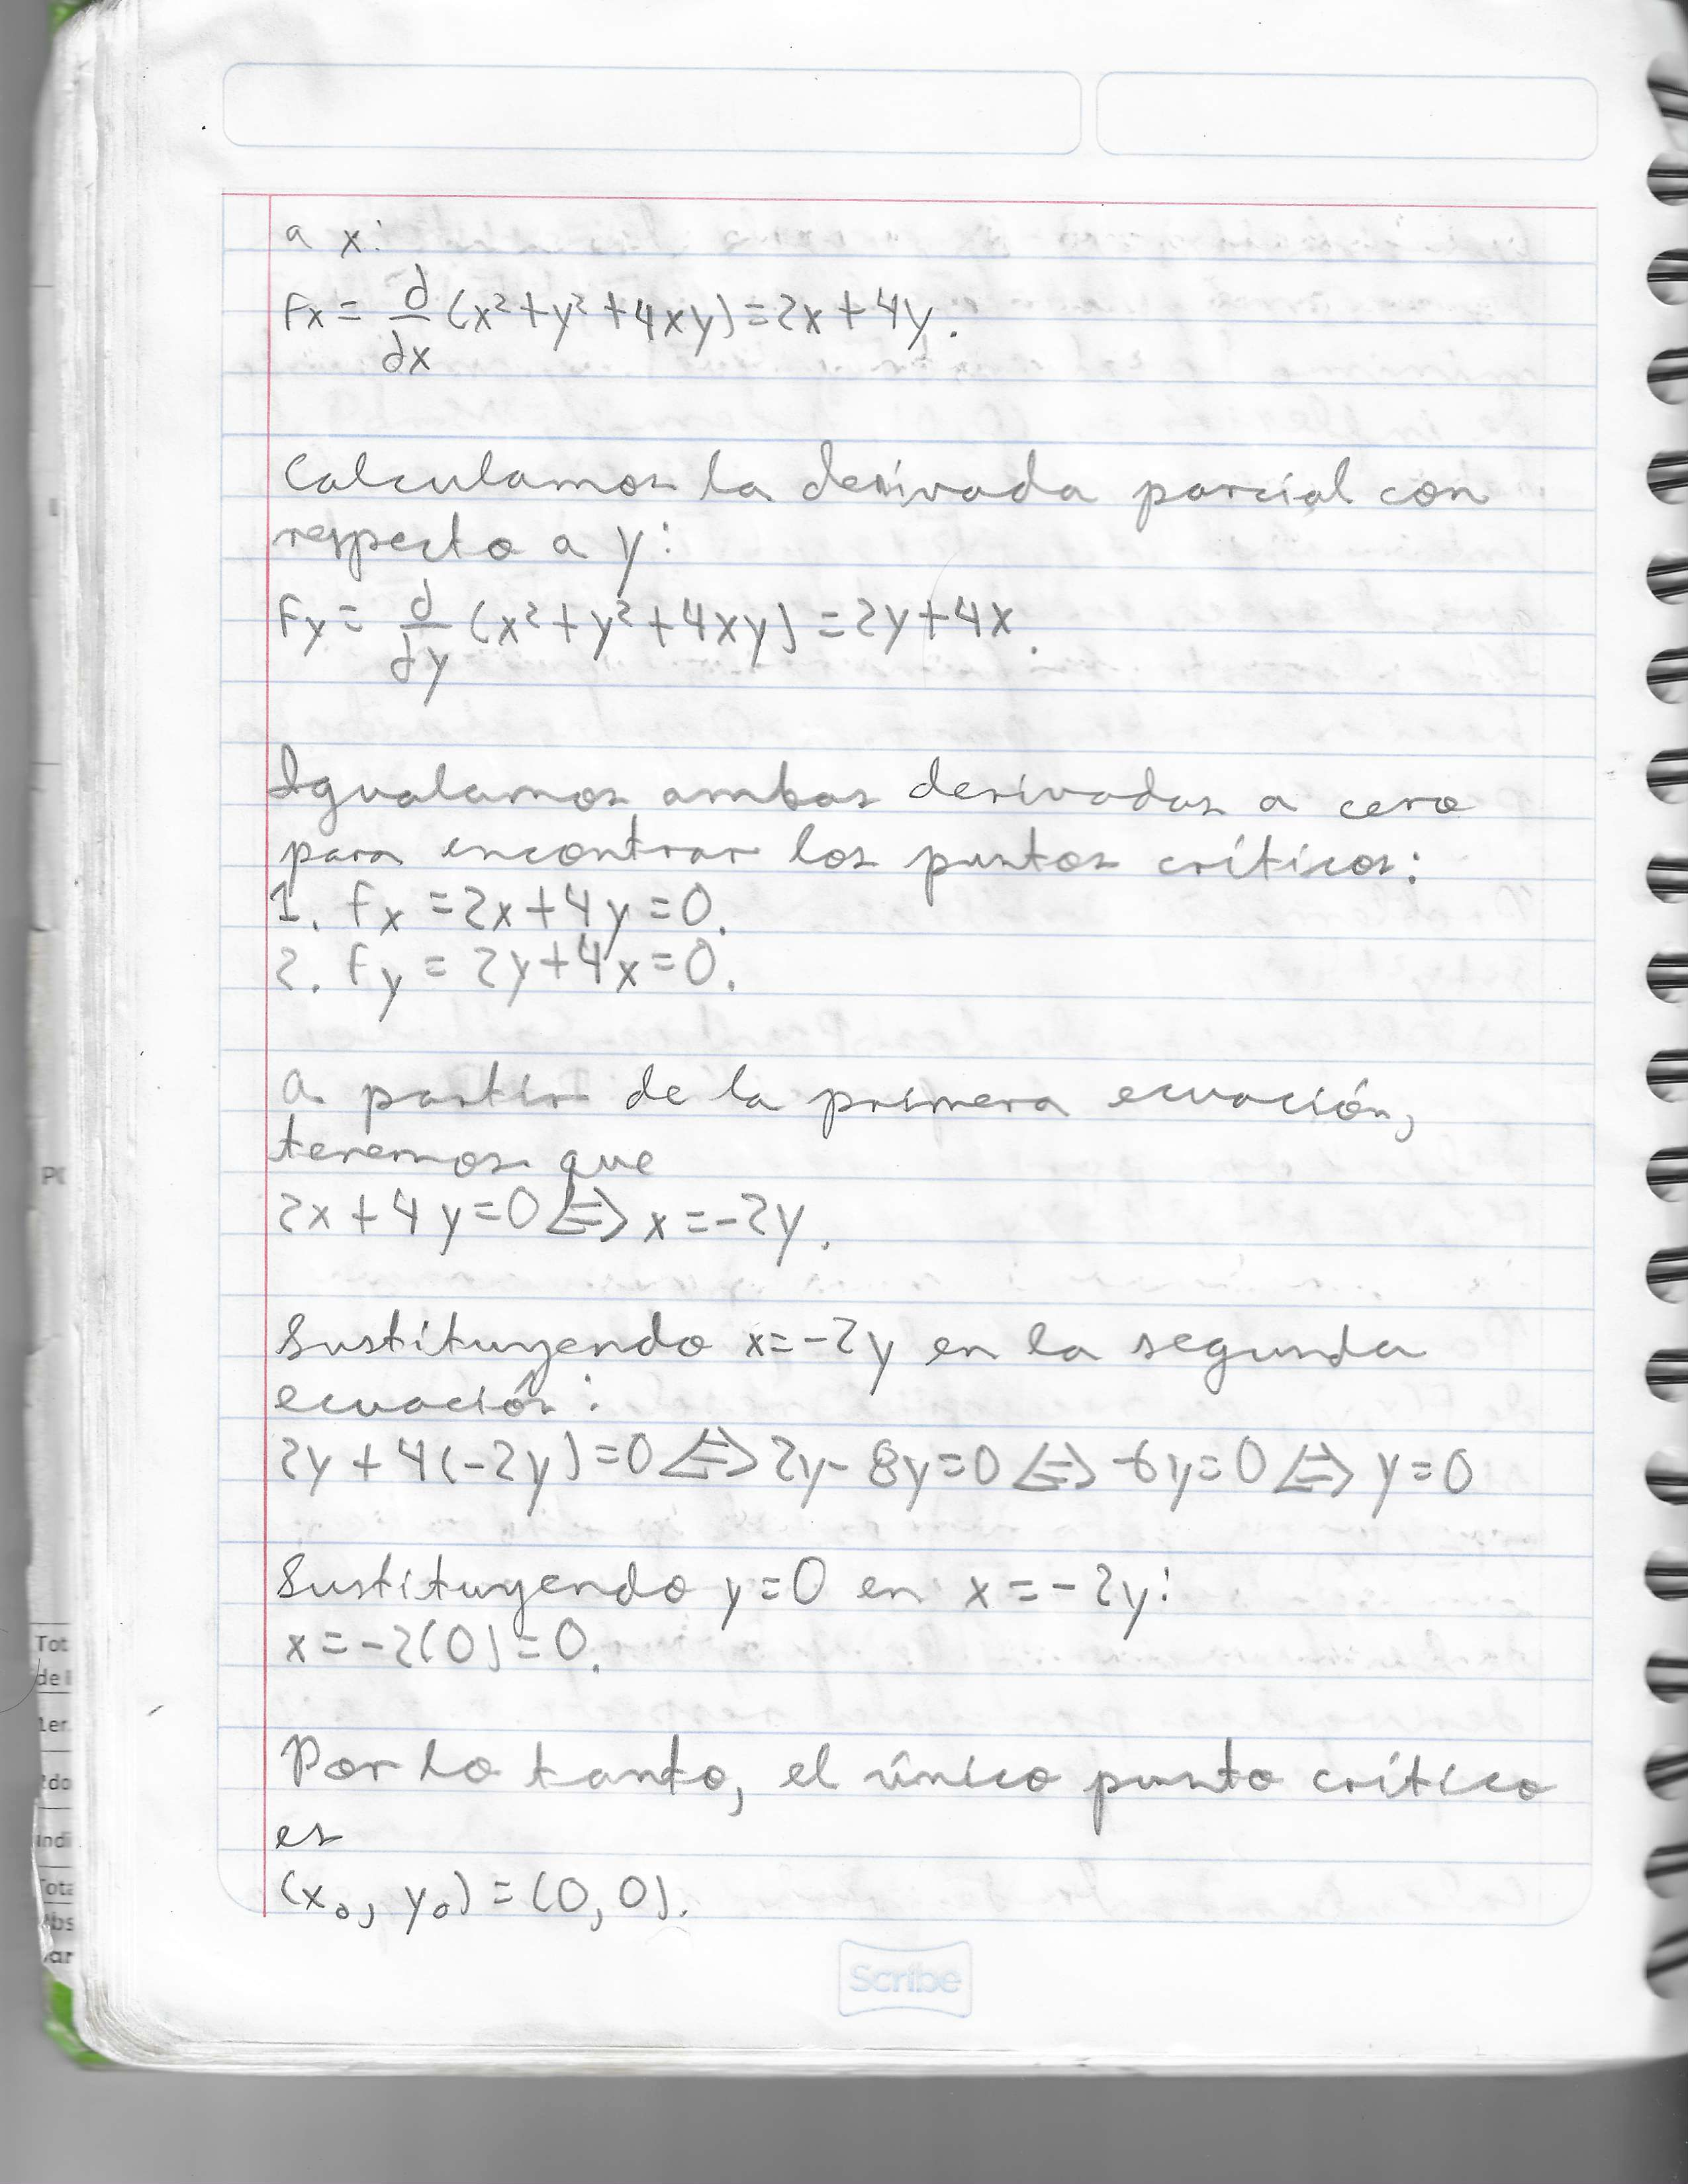
\includegraphics[width=0.8\textwidth]{imagenes/pagina5.png}
	\caption{Procedimiento a mano - Página 5}
	\label{fig:procedimiento_5}
\end{figure}

% Imagen 6
\begin{figure}[H]
	\centering
	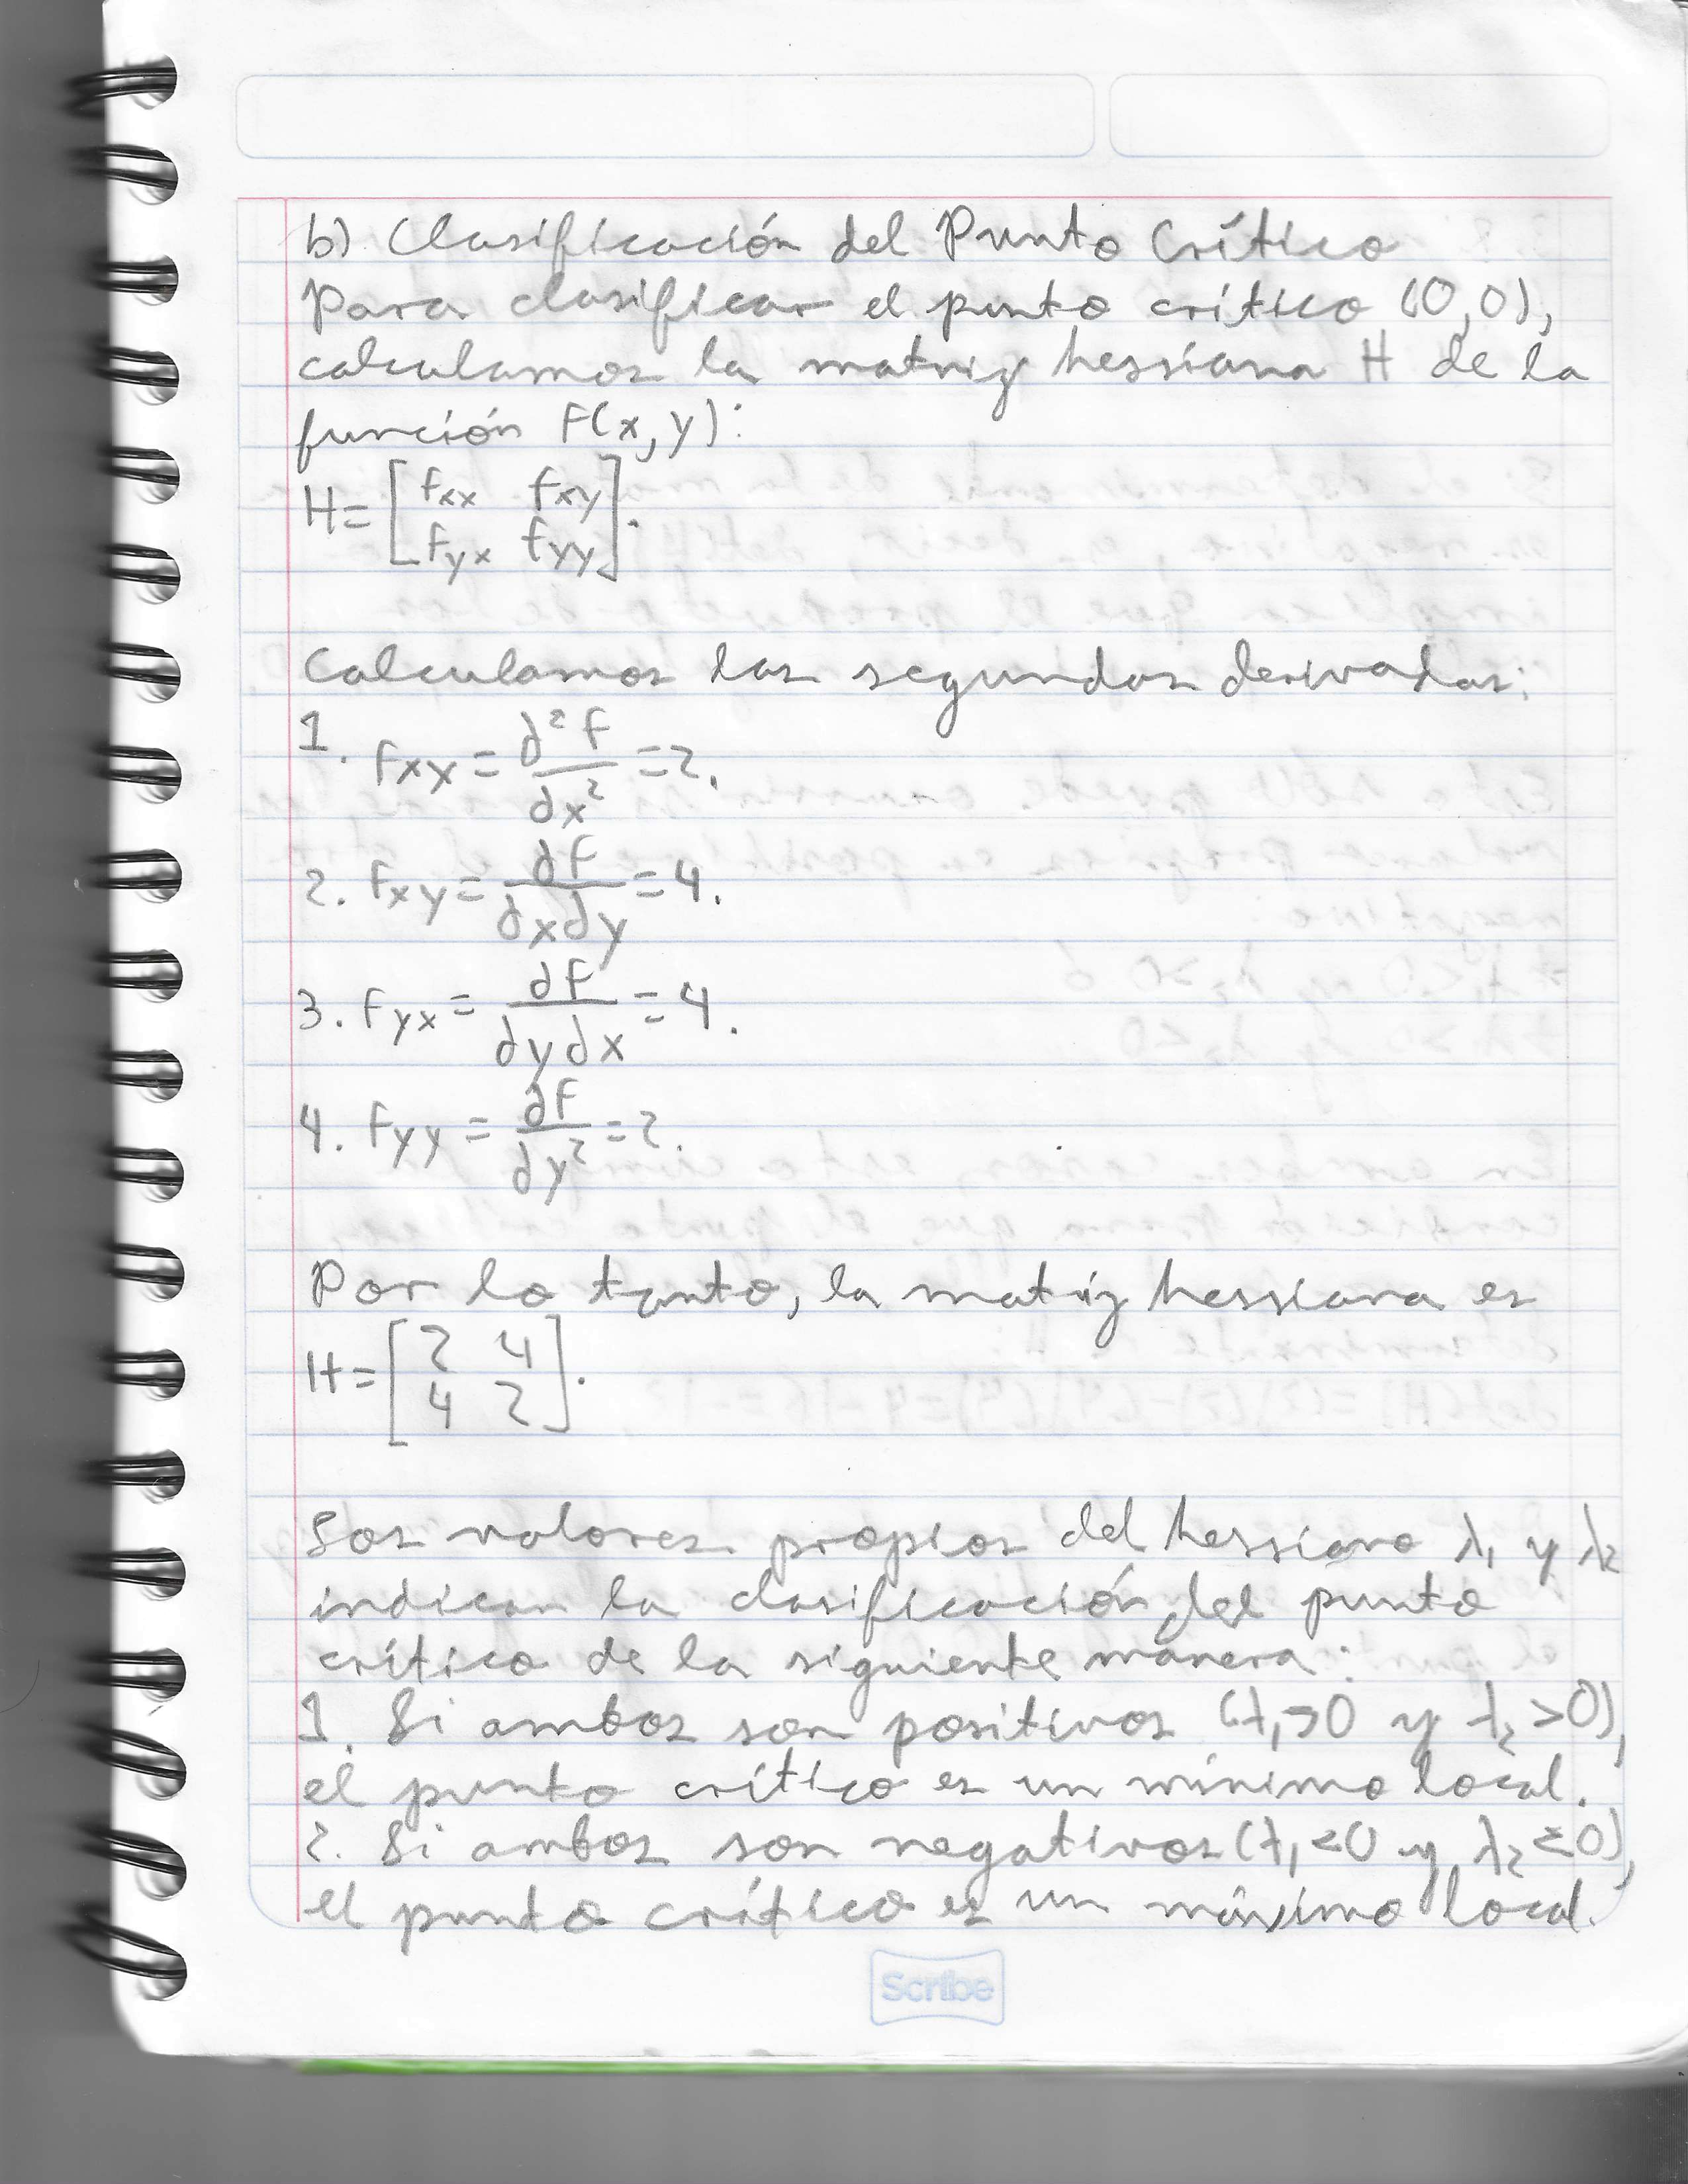
\includegraphics[width=0.8\textwidth]{imagenes/pagina6.png}
	\caption{Procedimiento a mano - Página 6}
	\label{fig:procedimiento_6}
\end{figure}

% Imagen 7
\begin{figure}[H]
	\centering
	\includegraphics[width=0.8\textwidth]{imagenes/pagina7.png}
	\caption{Procedimiento a mano - Página 7}
	\label{fig:procedimiento_7}
\end{figure}

\bibliography{actividad1}

\end{document}
